\thispagestyle{toancuabinone}
\pagestyle{toancuabi}
\everymath{\color{toancuabi}}
%\blfootnote{$^1$\color{toancuabi}Trường Liên cấp Hội nhập Quốc tế iSchool Quảng Trị.}
\graphicspath{{../toancuabi/pic/}}
\begingroup
\AddToShipoutPicture*{\put(0,616){\includegraphics[width=19.3cm]{../bannertoancuabi}}}  
\AddToShipoutPicture*{\put(60,492){\includegraphics[scale=1]{../tieude1.pdf}}}  
\centering
\endgroup
\vspace*{215pt} 

\definecolor{bulgarianrose}{rgb}{0.28, 0.02, 0.03}
\begin{multicols}{2}
	Câu lạc bộ toán học ``Unicorn Math Circle" (UMC) dành cho học sinh Tiểu học và THCS được Tạp chí Pi tổ chức từ năm $2019$, nhằm tìm kiếm và bồi dưỡng các học sinh có năng lực Toán học, tạo nguồn học sinh xuất sắc. Trong số này, tạp chí Pi giới thiệu đến bạn đọc đề thi tuyển sinh năm học $2023-2024$ dành cho các bạn học sinh lớp $4$.
	\vskip 0.1cm
	\textbf{\color{toancuabi}Bài $\pmb{1.}$} Dựa vào quy luật, hỏi hình nào trong số các hình $A$, $B$, $C$, $D$ là hình tiếp theo trong dãy sau:
	\begin{figure}[H]
		\vspace*{-5pt}
		\centering
		\captionsetup{labelformat= empty, justification=centering}
		\begin{tikzpicture}[toancuabi,scale=0.29]
			\fill[cackithi!50] (0,0) rectangle (1,1);
			\fill[cackithi!50] (2,0) rectangle (3,1);
			\fill[cackithi!50] (5,0) rectangle (6,1);
			\fill[cackithi!50] (11,0) rectangle (12,1);
			\draw (0,0) grid (1,1);
			\draw (2,0) grid (4,1);
			\draw (5,0) grid (7,1);
			\draw (5,1) grid (6,3);
			\draw (8,0) grid (13,1);
			\draw (11,1) grid (12,3);
			\draw (14,0.25) node {$?$};
		\end{tikzpicture}

		\vspace*{10pt}
		\begin{tikzpicture}[toancuabi,scale=0.29]
			\fill[cackithi!50] (3,0) rectangle (4,1);
			\fill[cackithi!50] (9,0) rectangle (10,1);
			\fill[cackithi!50] (15,0) rectangle (16,1);
			\fill[cackithi!50] (23,0) rectangle (24,1);
			\draw (0,0) grid (5,1);
			\draw (3,-3) grid (4,3);
			\draw (6,0) grid (11,1);
			\draw (9,-4) grid (10,3);
			\draw (12,0) grid (19,1);
			\draw (15, 1) grid (16,3);
			\draw (20,0) grid (25,1);
			\draw (23,-2) grid (24,3);
			
			\draw (3.5,-5) node{$A$};
			\draw (9.5,-5) node{$B$};
			\draw (15.5,-5) node{$C$};
			\draw (21.5,-5) node{$D$};
		\end{tikzpicture}
		\vspace*{-15pt}
	\end{figure}
	\textbf{\color{toancuabi}Bài $\pmb{2.}$} Một cặp số có hai chữ số như $18$ và $81$ được gọi là cặp \textit{bạn thân} vì chúng có chữ số hàng chục và chữ số hàng đơn vị đổi chỗ cho nhau. Hỏi có bao nhiêu cặp bạn thân mà tổng của chúng bằng $99$?
	\vskip 0.1cm
	\textbf{\color{toancuabi}Bài $\pmb{3.}$} Bạn Ngọc được tặng một thanh sô--cô--la hình trái tim. Mỗi ô vuông có trọng lượng $8$g. Hỏi thanh sô--cô--la có khối lượng bằng bao nhiêu?
	\begin{figure}[H]
		\vspace*{-5pt}
		\centering
		\captionsetup{labelformat= empty, justification=centering}
		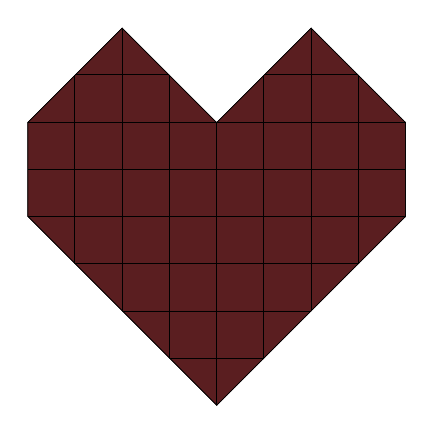
\begin{tikzpicture}[scale=0.6]
			\clip (0,0) - ++(0,2) - ++(2,4) - ++(4,2) - ++(6,4) - ++(8,2) - ++(8,0) - ++(4,-4) -- cycle;;
			\draw[fill=bulgarianrose!90] (0,0) - ++(0,2) - ++(2,4) - ++(4,2) - ++(6,4) - ++(8,2) - ++(8,0) - ++(4,-4) -- cycle;
			\draw (0,0) - ++(0,2) - ++(2,4) - ++(4,2) - ++(6,4) - ++(8,2) - ++(8,0) - ++(4,-4) -- cycle;
			\draw (0,-4) grid (8,4);
		\end{tikzpicture}
		\vspace*{-5pt}
	\end{figure}
	\textbf{\color{toancuabi}Bài $\pmb{4.}$} Trong hình vẽ sau, mỗi miền tô $1$ màu, không có $2$ miền nào cùng màu. Có bao nhiêu miền nằm trong ít nhất $3$ hình tròn?	 
	\begin{figure}[H]
		\vspace*{-5pt}
		\centering
		\captionsetup{labelformat= empty, justification=centering}
		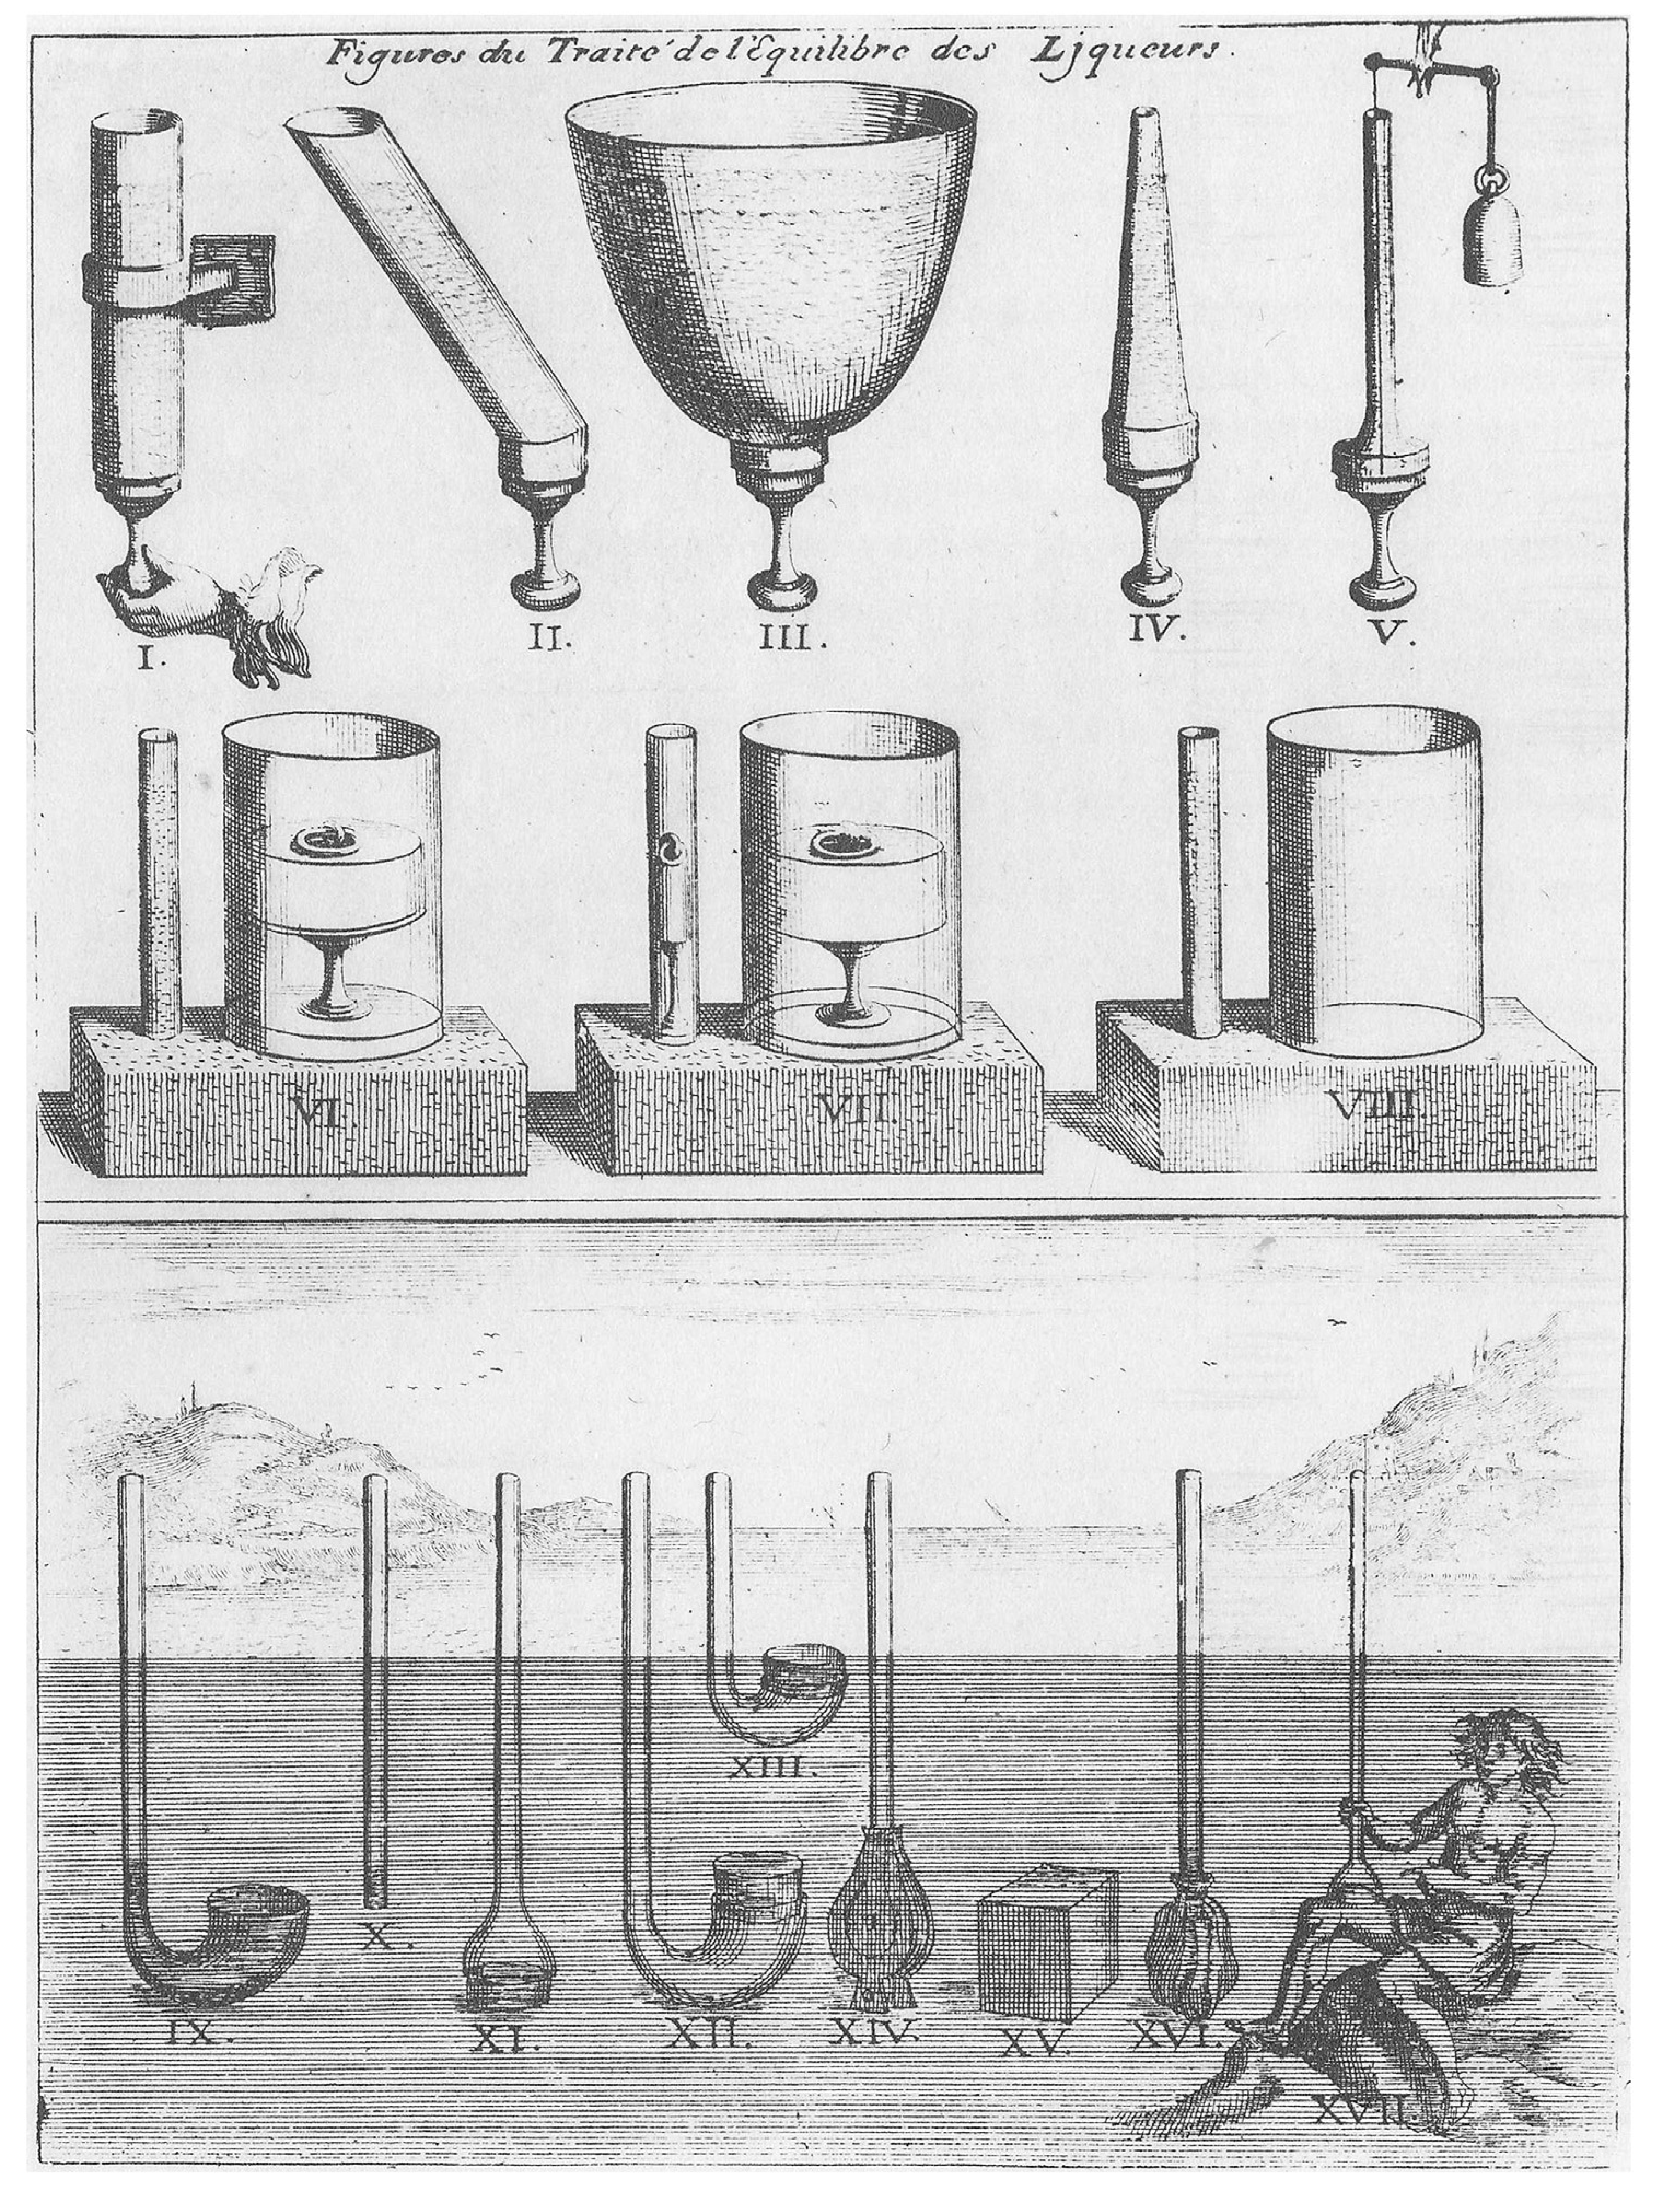
\includegraphics[width= 0.65\linewidth]{2}
%		\caption{\small\textit{\color{}}}
		\vspace*{-5pt}
	\end{figure}
	\textbf{\color{toancuabi}Bài $\pmb{5.}$} Số $1995$ được xếp bằng các que diêm như hình dưới đây. An dịch chuyển đúng $1$ que diêm để nhận được số lớn nhất có thể. Hỏi số đó bằng bao nhiêu?
	\begin{figure}[H]
		\vspace*{-5pt}
		\centering
		\captionsetup{labelformat= empty, justification=centering}
		\includegraphics[width= 1\linewidth]{3}
%		\caption{\small\textit{\color{}}}
		\vspace*{-15pt}
	\end{figure}
	\textbf{\color{toancuabi}Bài $\pmb{6.}$} Như hình vẽ, có $9$ ô vuông nhỏ, vẽ một đường thẳng, hỏi đường thẳng này đi qua nhiều nhất bao nhiêu ô vuông nhỏ?
	\begin{figure}[H]
		\vspace*{-5pt}
		\centering
		\captionsetup{labelformat= empty, justification=centering}
		\begin{tikzpicture}[scale=1.2]
			\draw[fill=diendantoanhoc!50] (0,0) rectangle (1,1);
			\draw[fill=gocco!50] (0,1) rectangle (1,2);
			\draw[fill=toancuabi!50] (0,2) rectangle (1,3);
			\draw[fill=cackithi!50] (1,0) rectangle (2,1);
			\draw[fill=thachthuctoanhoc!50] (1,1) rectangle (2,2);
			\draw[fill=duongvaotoanhoc!50] (1,2) rectangle (2,3);
			\draw[fill=quantoan!80] (2,0) rectangle (3,1);
			\draw[fill=lichsutoanhoc!50] (2,1) rectangle (3,2);
			\draw[fill=timhieukhoahoc!60] (2,2) rectangle (3,3);
			\draw (0,0) grid (3,3);
		\end{tikzpicture}
		\vspace*{-5pt}
	\end{figure}
	\textbf{\color{toancuabi}Bài $\pmb{7.}$} Trong hình vẽ bên dưới, hình ngôi sao lớn được chia thành các hình tam giác có chu vi bằng $7$, các hình tứ giác có chu vi bằng $18$ và một hình ngôi sao nhỏ có chu vi bằng $3$. Tìm chu vi của hình ngôi sao lớn ban đầu.
	\begin{figure}[H]
		\vspace*{-5pt}
		\centering
		\captionsetup{labelformat= empty, justification=centering}
		\includegraphics[width= 0.7\linewidth]{5}
%		\caption{\small\textit{\color{}}}
%		\vspace*{-10pt}
	\end{figure}
	\textbf{\color{toancuabi}Bài $\pmb{8.}$} Trong siêu thị có sự kiện ra mắt $1$ loại kem mới, để quảng cáo loại kem này, họ cho phép cứ $2$ cái vỏ que kem đổi được $1$ cây kem, bạn Bảo Châu mua $10$ que kem, vậy bạn ấy thực sự có thể ăn được nhiều nhất bao nhiêu que kem?
	\vskip 0.1cm
	\textbf{\color{toancuabi}Bài $\pmb{9.}$} Một hình vuông to được chia thành các hình vuông nhỏ hơn với nhiều kích cỡ, trong đó một số được tô màu hồng như hình vẽ. Biết diện tích phần màu trắng của hình vuông là $180$. Tìm diện tích phần màu đen của hình vuông.
	\begin{figure}[H]
	\vspace*{-5pt}
	\centering
	\captionsetup{labelformat= empty, justification=centering}
	\begin{tikzpicture}[scale=0.55, cackithi]
		\fill[fill=toancuabi] (-2.,7.) -- (-2.,5.5) -- (-0.5,5.5) -- (-0.5,7.) -- cycle;
		\fill[fill=toancuabi] (-0.5,5.5) -- (-0.5,4.) -- (1.,4.) -- (1.,5.5) -- cycle;
		\fill[fill=toancuabi] (1.,7.) -- (1.,5.) -- (3.,5.) -- (3.,7.) -- cycle;
		\fill[fill=toancuabi] (5.,7.) -- (5.,5.) -- (7.,5.) -- (7.,7.) -- cycle;
		\fill[fill=toancuabi] (4.,5.) -- (4.,4.) -- (5.,4.) -- (5.,5.) -- cycle;
		\fill[fill=toancuabi] (3.,4.) -- (3.,3.) -- (4.,3.) -- (4.,4.) -- cycle;
		\fill[fill=toancuabi] (5.,3.) -- (5.,1.) -- (7.,1.) -- (7.,3.) -- cycle;
		\fill[fill=toancuabi] (1.,3.) -- (1.,1.) -- (3.,1.) -- (3.,3.) -- cycle;
		\fill[fill=toancuabi] (4.,1.) -- (4.,-0.5) -- (5.5,-0.5) -- (5.5,1.) -- cycle;
		\fill[fill=toancuabi] (5.5,-0.5) -- (5.5,-2.) -- (7.,-2.) -- (7.,-0.5) -- cycle;
		\fill[fill=toancuabi] (-2.,1.) -- (-2.,-2.) -- (1.,-2.) -- (1.,1.) -- cycle;
		\draw  (3.,5.)-- (5.,5.);
		\draw  (5.,5.)-- (5.,3.);
		\draw  (5.,3.)-- (3.,3.);
		\draw  (3.,3.)-- (3.,5.);
		\draw  (4.,5.)-- (4.,3.);
		\draw  (3.,4.)-- (5.,4.);
		\draw  (7.,5.)-- (7.,3.);
		\draw  (7.,3.)-- (5.,3.);
		\draw  (3.,5.)-- (1.,5.);
		\draw  (1.,5.)-- (1.,3.);
		\draw  (1.,3.)-- (3.,3.);
		\draw  (1.,3.)-- (1.,1.);
		\draw  (1.,1.)-- (7.,1.);
		\draw  (7.,1.)-- (7.,3.);
		\draw  (5.,3.)-- (5.,1.);
		\draw  (3.,3.)-- (3.,1.);
		\draw  (1.,5.)-- (1.,7.);
		\draw  (1.,7.)-- (7.,7.);
		\draw  (7.,7.)-- (7.,5.);
		\draw  (5.,5.)-- (5.,7.);
		\draw  (3.,5.)-- (3.,7.);
		\draw  (1.,7.)-- (-2.,7.);
		\draw  (-2.,7.)-- (-2.,1.);
		\draw  (1.,4.)-- (-2.,4.);
		\draw  (-2.,-2.)-- (7.,-2.);
		\draw  (7.,-2.)-- (7.,1.);
		\draw  (4.,1.)-- (4.,-2.);
		\draw  (-2.,7.)-- (-2.,5.5);
		\draw  (-2.,5.5)-- (-0.5,5.5);
		\draw  (-0.5,5.5)-- (-0.5,7.);
		\draw  (-0.5,7.)-- (-2.,7.);
		\draw  (-0.5,5.5)-- (-0.5,4.);
		\draw  (-0.5,4.)-- (1.,4.);
		\draw  (1.,4.)-- (1.,5.5);
		\draw  (1.,5.5)-- (-0.5,5.5);
		\draw  (1.,7.)-- (1.,5.);
		\draw  (1.,5.)-- (3.,5.);
		\draw  (3.,5.)-- (3.,7.);
		\draw  (3.,7.)-- (1.,7.);
		\draw  (5.,7.)-- (5.,5.);
		\draw  (5.,5.)-- (7.,5.);
		\draw  (7.,5.)-- (7.,7.);
		\draw  (7.,7.)-- (5.,7.);
		\draw  (4.,5.)-- (4.,4.);
		\draw  (4.,4.)-- (5.,4.);
		\draw  (5.,4.)-- (5.,5.);
		\draw  (5.,5.)-- (4.,5.);
		\draw  (3.,4.)-- (3.,3.);
		\draw  (3.,3.)-- (4.,3.);
		\draw  (4.,3.)-- (4.,4.);
		\draw  (4.,4.)-- (3.,4.);
		\draw  (5.,3.)-- (5.,1.);
		\draw  (5.,1.)-- (7.,1.);
		\draw  (7.,1.)-- (7.,3.);
		\draw  (7.,3.)-- (5.,3.);
		\draw  (1.,3.)-- (1.,1.);
		\draw  (1.,1.)-- (3.,1.);
		\draw  (3.,1.)-- (3.,3.);
		\draw  (3.,3.)-- (1.,3.);
		\draw  (4.,1.)-- (4.,-0.5);
		\draw  (4.,-0.5)-- (5.5,-0.5);
		\draw  (5.5,-0.5)-- (5.5,1.);
		\draw  (5.5,1.)-- (4.,1.);
		\draw  (5.5,-0.5)-- (5.5,-2.);
		\draw  (5.5,-2.)-- (7.,-2.);
		\draw  (7.,-2.)-- (7.,-0.5);
		\draw  (7.,-0.5)-- (5.5,-0.5);
		\draw  (-2.,1.)-- (-2.,-2.);
		\draw  (-2.,-2.)-- (1.,-2.);
		\draw  (1.,-2.)-- (1.,1.);
		\draw  (1.,1.)-- (-2.,1.);
	\end{tikzpicture}
	\vspace*{-5pt}
	\end{figure}
	\textbf{\color{toancuabi}Bài $\pmb{10.}$} Hai bạn Nam và Dương đi chợ sách và nhìn thấy cuốn tạp chí Pi. Nam muốn mua $1$ cuốn nhưng thiếu $12$ nghìn đồng. Dương muốn mua $1$ cuốn nhưng thiếu $23$ nghìn đồng. Nếu $2$ bạn chung tiền mua thì vừa đủ mua $1$ cuốn. Hỏi cuốn tạp chí Pi giá bao nhiêu tiền?
	\end{multicols}
	\newpage
	\begin{multicols}{2}
	\textbf{\color{toancuabi}Lời giải.}
	\vskip 0.1cm
	\textbf{\color{toancuabi}Bài $\pmb{1.}$} Ta thấy nếu lấy ô vuông được tô màu làm tâm, thì theo ngược chiều kim đồng hồ số các ô vuông kề với tâm sẽ tăng dần: $1,2,3,4$. Do đó hình $B$ là hình tiếp theo trong dãy.
	\vskip 0.1cm
	\textbf{\color{toancuabi}Bài $\pmb{2.}$} Ta có thể thấy ngay cặp số bạn thân có tổng bằng $99$ thì mỗi số trong cặp có tổng chữ số hàng chục và hàng đơn vị bằng $9$. Do $9 = 1+8 = 2+7 = 3+6 = 4+5$ nên ta có $4$ cặp số số bạn thân thỏa mãn là: $18-81$, $27-72$, $26-63$, $45-54$.
	\vskip 0.1cm
	\textbf{\color{toancuabi}Bài $\pmb{3.}$} Thanh sô--cô--la hình trái tim được ghép từ $32$ miếng ô vuông diện tích và $16$ miếng nửa ô vuông. Sau khi ghép các nửa ô vuông lại với nhau, thì ta thấy thanh sô--cô--la gồm $40$ ô. Do đó khối lượng của thanh sô--cô--la là: $4\times 80=320 \text{ (g)}$.
	\vskip 0.1cm
	\textbf{\color{toancuabi}Bài $\pmb{4.}$} Đánh số các miền như trong hình dưới đây. Ta thấy các miền $4$, $5$, $10$, $9$ và $7$ nằm trong ít nhất $3$ hình tròn. Do đó có $5$ miền thỏa mãn đề bài.
	\begin{figure}[H]
		\vspace*{-5pt}
		\centering
		\captionsetup{labelformat= empty, justification=centering}
		\includegraphics[width= 0.7\linewidth]{7}
%		\caption{\small\textit{\color{}}}
		\vspace*{-10pt}
	\end{figure}
	\textbf{\color{toancuabi}Bài $\pmb{5.}$} Bạn An di chuyển một que diêm từ chữ số $9$ hàng chục sang chữ số $1$ hàng nghìn và được số lớn nhất là:  
	\begin{figure}[H]
		\vspace*{-5pt}
		\centering
		\captionsetup{labelformat= empty, justification=centering}
		\includegraphics[width= 1\linewidth]{8}
%		\caption{\small\textit{\color{}}}
		\vspace*{-15pt}
	\end{figure}
	\textbf{\color{toancuabi}Bài $\pmb{6.}$} Ta vẽ đường thẳng như hình dưới đây, khi đó đường thẳng đi qua nhiều nhất $5$ hình vuông nhỏ.
	\begin{figure}[H]
		\vspace*{-5pt}
		\centering
		\captionsetup{labelformat= empty, justification=centering}
		\begin{tikzpicture}[scale=1.2]
			\draw[fill=diendantoanhoc!50] (0,0) rectangle (1,1);
			\draw[fill=gocco!50] (0,1) rectangle (1,2);
			\draw[fill=toancuabi!50] (0,2) rectangle (1,3);
			\draw[fill=cackithi!50] (1,0) rectangle (2,1);
			\draw[fill=thachthuctoanhoc!50] (1,1) rectangle (2,2);
			\draw[fill=duongvaotoanhoc!50] (1,2) rectangle (2,3);
			\draw[fill=quantoan!80] (2,0) rectangle (3,1);
			\draw[fill=lichsutoanhoc!50] (2,1) rectangle (3,2);
			\draw[fill=timhieukhoahoc!60] (2,2) rectangle (3,3);
			\draw (0,0) grid (3,3);
			\draw[line width= 2pt, toanhocdoisong] (0.25,3.5) -- (3.5,0); 
		\end{tikzpicture}
%		\vspace*{-5pt}
	\end{figure}
	\textbf{\color{toancuabi}Bài $\pmb{7.}$} Tổng các cạnh của các hình tứ giác mà không phải là cạnh của ngôi sao lớn là:
	\begin{align*}
		7\times 5-3 = 32 \text{ (đơn vị).}
	\end{align*}
	Vậy chu vi của ngôi sao lớn ban đầu là:
	\begin{align*}
		18\times 5-32 = 58 \text{ (đơn vị).}
	\end{align*}
	\textbf{\color{toancuabi}Bài $\pmb{8.}$}  Đầu tiên bạn Châu đổi được $10:2=5$ (que kem). Với $5$ que kem mới này bạn đổi được $5:2=2$ que kem và dư $1$ vỏ que kem. Với $2$ vỏ que kem bạn Châu lại tiếp tục đổi được $1$ que kem. Cuối cùng $1$ vỏ que kem này và $1$ vỏ que kem còn thừa trước đó, bạn lại đổi được $1$ que kem nữa. Vậy tổng cộng bạn Châu được ăn số que kem là: 
	\begin{align*}
		10+5+2+1+1=19 \text{ (que kem).}
	\end{align*}
	\textbf{\color{toancuabi}Bài $\pmb{9.}$} Bằng cách ghép các phần được tô hồng như trong các minh họa dưới đây, ta thấy phần tô hồng gồm $4$ ô vuông nhỏ và phần màu trắng gồm $5$ ô vuông nhỏ.
	\begin{figure}[H]
		\vspace*{-5pt}
		\centering
		\captionsetup{labelformat= empty, justification=centering}
		\includegraphics[width= 1\linewidth]{10a.pdf}
		%		\caption{\small\textit{\color{}}}
		\vspace*{-15pt}
	\end{figure}
	Như vậy diện tích một ô vuông nhỏ là: 
	\begin{align*}
		180:5 = 36 \text{ (đơn vị).}
	\end{align*}
	Do đó diện tích phần được tô đen là: 
	\begin{align*}
		36\times 4 = 144 \text{ (đơn vị).}
	\end{align*}
	\textbf{\color{toancuabi}Bài $\pmb{10.}$} Vì hai bạn chung tiền mua thì vừa đủ $1$ cuốn tạp chí Pi, nên số tiền mà Nam còn thiếu chính là số tiền mà Dương có, số tiền mà Dương thiếu chính là số tiền mà Nam có. Vậy Dương có $12$ nghìn, Nam có $23$ nghìn. Vậy cuốn tạp chí Pi giá $12+23=35$ (nghìn).
\end{multicols}
\newpage
\graphicspath{{../toancuabi/pic/}}
\begingroup
\AddToShipoutPicture*{\put(110,645){\includegraphics[scale=1]{../tieude.pdf}}}  
\centering
\endgroup
\vspace*{60 pt} 
\begin{multicols}{2}
	Thám tử Xuân Phong đôi khi phải đột nhập vào những nơi hoang vắng, kỳ bí để tìm ra được dấu tích của những kẻ gây án. Một lần nọ, sau bao ngày cải trang để bám sát theo dõi manh mối, thám tử biết tên trùm tội phạm đang trốn tránh trong một ngôi nhà hẻo lánh ở ngoại ô. Vừa đến trước cửa của ngôi nhà gỗ cổ kính, Xuân Phong gặp một bà lão với đôi mắt tinh anh nhìn mình với vẻ bí mật ``Thám tử đó phải không, tôi nhận ngay ra ngài, dù ngài đã cải trang rất kỹ. Phải chăng thám tử đang đi tìm tên trùm? Hắn đang ngồi dưới kia, trong căn phòng cùng những người trong hiệp hội Thương Gia, nhưng vô cùng nguy hiểm nếu ngài dùng vũ lực ở đây để bắt hắn. Tôi mách ngài nhé, ở dưới đó, có 10 người, có lão trùm và những kẻ đồng phạm cùng lão, là những kẻ luôn nói dối, nhưng cũng có thể có cả những người lương thiện, luôn nói thật, ở ngay bên cạnh. Ngài hãy dùng trí thông minh của mình, chỉ được hỏi rất hạn chế câu hỏi để phán đoán ra những kẻ phạm tội là ai. Ngài hỏi nhiều câu hơn sẽ nguy hiểm cho cả những Thương gia lương thiện có thể có mặt ở đó. Và ngài hãy hứa với bà lão này sẽ đảm bảo an toàn cho tôi và gia đình, vì tôi đã liều mình thông báo tin mật này với Thám tử".
	\vskip 0.1cm
	Theo lời bà lão mách bảo, Xuân Phong lần theo một chiếc cầu thang cũ nát và đi xuống một căn phòng khuất dưới tầng hầm. Vừa mở cửa ra, thám tử đã thấy có 10 người ăn mặc chỉnh tề như nhau, ngồi nghiêm trang quanh một chiếc bàn hình thập giác đều, mỗi người ngồi tại đỉnh của hình thập giác. Ánh sáng lờ mờ trong phòng đủ chiếu rõ dòng chữ ``Cuộc họp thường niên Hiệp hội Thương gia -- Khu vực Duyên Hải". Thật khó để xác định ai là kẻ nói dối trong số họ, vì vẻ ngoài họ đều giống như những Thương Gia thường gặp: quyền lực, sắc sảo và oai vệ.
	\begin{figure}[H]
		\centering
		\vspace*{-5pt}
		\captionsetup{labelformat= empty, justification=centering}
		\includegraphics[width=1\linewidth]{xp}
		\vspace*{-15pt}
	\end{figure}
	Theo quy định của Hiệp hội Thương gia dành cho những người ngoài, qua lời rỉ tai của bà lão, Thám tử có thể đứng dậy bước tới một nơi bất kỳ nào đó trong căn phòng và chỉ được hỏi câu hỏi ``Khoảng cách từ chỗ tôi đứng đến người nói dối gần nhất trong số các anh là bao nhiêu?" cho tất cả những người trong phòng. Sau đó, mỗi người trong số $10$ người ngồi xung quanh bàn sẽ trả lời Thám tử, lúc này đã cải trang thành một Thương gia muốn gia nhập Hiệp hội. Thám tử không được phép đứng lên mặt bàn và tất cả mọi người, kể cả Thám tử, đều được phép dùng thước để đo khoảng cách tuỳ ý. Ta cũng được biết rằng ngoài $10$ người và Thám tử, trong phòng không còn có người lạ nào khác, hơn nữa $10$ người đều biết rõ ai trong số họ là nói thật và ai trong số họ là nói dối. Em hãy cho biết Xuân Phong có thể sử dụng ít nhất bao nhiêu câu hỏi như trên để biết chắc chắn ai trong số những người ngồi quanh bàn là nói~dối?
\end{multicols}
\newpage
\begingroup
\AddToShipoutPicture*{\put(115,670){\includegraphics[scale=1]{../tieude11.pdf}}} 
\centering
\endgroup
\vspace*{35pt}

\begin{multicols}{2}
	$\pmb{1.}$ Tuấn và Tú cùng tham gia một giải thi đấu cờ vua cùng các bạn học sinh khác trong trường. Hai bạn tổng cộng ghi được $6{.}5$ điểm, trong khi tất cả các bạn học sinh còn lại đều ghi được số điểm bằng nhau. Hỏi có tất cả bao nhiêu học sinh tham gia giải cờ vua đó? (Biết rằng trong giải thi đấu, mỗi người tham gia thi đấu đúng một ván với mỗi người còn lại, ghi được $1$ điểm sau mỗi trận thắng, $0{.}5$ điểm sau mỗi trận hoà và $0$ điểm sau mỗi trận thua).
	\begin{figure}[H]
		\centering
		\vspace*{-5pt}
		\captionsetup{labelformat= empty, justification=centering}
		\includegraphics[width=1\linewidth]{Hinh1}
		\vspace*{-20pt}
	\end{figure}
	$\pmb{2.}$ 	Lớp $6$A gồm $22$ bạn chia thành hai đội Xanh gồm các bạn nam và Đỏ gồm các bạn nữ để tổ chức thi tài đối đáp trả lời thông minh. Đầu tiên, bạn Hoa ở nhóm Đỏ đối đáp với $6$ bạn nam ở nhóm Xanh và giành chiến thắng. Tiếp theo, bạn Mai ở nhóm Đỏ đối đáp với $7$ bạn nam ở nhóm Xanh và cũng giành chiến thắng. Tiếp tục bạn Huệ ở nhóm Đỏ cũng chiến thắng $8$ bạn nam ở nhóm Xanh. Cứ tiếp tục như vậy, cuối cùng bạn Hà ở nhóm Đỏ đã đối đáp thông minh với toàn bộ các bạn nam ở nhóm Xanh và giành chiến thắng chung cuộc. Hỏi trong lớp có tất cả bao nhiêu bạn nam?
	\begin{figure}[H]
		\centering
		\vspace*{-5pt}
		\captionsetup{labelformat= empty, justification=centering}
		\includegraphics[width=1.01\linewidth]{Hinh2}
		\vspace*{-5pt}
	\end{figure}
	$\pmb{3.}$ 	Có ba chủ doanh nghiệp tới thăm trường học cũ của mình, mang theo một số món quà với dự định sẽ trao tặng cho một nửa số học sinh đang học ở đó. Khi tất cả $252$ em học sinh được mời xếp thành một hàng ngang, chủ doanh nghiệp thứ nhất tặng quà cho mỗi em đứng thứ tư trong hàng (các em ở số thứ tự $4,8,12,$ v.v\ldots). Chủ doanh nghiệp thứ hai lại tặng quà cho mỗi em đứng thứ bảy (các em ở số thứ tự $7,14,21$, v.v\ldots). Chủ doanh nghiệp thứ ba lại trao tặng quà cho mỗi em đứng thứ $11$ (các em ở số thứ tự $11,22,33$, v.v\ldots). Hỏi có bao nhiêu em học sinh nhận được quà và bao nhiêu em không nhận được quà?
	\begin{figure}[H]
		\centering
		\vspace*{-5pt}
		\captionsetup{labelformat= empty, justification=centering}
		\includegraphics[width=1\linewidth]{Hinh3}
		\vspace*{-15pt}
	\end{figure}
	$\pmb{4.}$ 	Có ba nhà tài trợ quyết định giúp đỡ một tạp chí khoa học thường thức với tên gọi là Phi. Nhà tài trợ Quốc trao tặng một khoản tiền tính bằng dollar gồm có $4$ chữ số: $2$ chữ số đứng trước dấu phẩy, và hai chữ số sau dấu phẩy, trong đó số cent lẻ (tức là hai chữ số đứng sau dấu phẩy) bằng với đúng số dollar chẵn (tức là hai chữ số đứng trước dấu phẩy; ta nhớ lại $100$ cent $= 1$ dollar). Nhà tài trợ Minh tặng số tiền với số dollar chẵn lớn hơn $3$ dollar so với số dollar chẵn mà nhà tài trợ Quốc đã tặng nhưng số cent lẻ lại ít hơn $8$ lần số cent lẻ của nhà tài trợ Quốc. Nhà tài trợ Vũ hào phóng đem tặng số tiền bằng $1/7$ tổng số tiền của hai nhà tài trợ Quốc và Minh đã trao cộng lại. Hỏi số tiền ủng hộ của ba nhà tài trợ cho tạp chí Phi là bao nhiêu?
	\begin{figure}[H]
		\centering
%		\vspace*{-5pt}
		\captionsetup{labelformat= empty, justification=centering}
		\includegraphics[width=1\linewidth]{Hinh4}
		\vspace*{-20pt}
	\end{figure}
	\vskip 0.1cm
	$\pmb{5.}$ 	Trên hòn đảo Ngọc ở giữa một đại dương xanh ngắt nọ có $100$ thổ dân sinh sống, một số người trong họ luôn nói dối, còn những người còn lại luôn nói thật. Mỗi một thổ dân thờ phụng đúng một trong ba loại thần: thần Mặt trời, thần Mặt trăng hoặc thần Đất. Người ta hỏi mỗi thổ dân ba câu hỏi sau đây:
	\begin{figure}[H]
		\centering
		\vspace*{-5pt}
		\captionsetup{labelformat= empty, justification=centering}
		\includegraphics[width=1\linewidth]{Hinh5}
		\vspace*{-15pt}
	\end{figure}
	$1.$ Ông (bà) có thờ phụng thần Mặt trời hay không?
	\vskip 0.1cm
	$2.$ Ông (bà) có thờ phụng thần Mặt trăng hay không?
	\vskip 0.1cm
	$3.$ Ông (bà) có thờ phụng thần Đất hay không?
	\vskip 0.1cm
	Có $60$ người trả lời khẳng định ``có" với câu hỏi thứ nhất, $40$ người trả lời khẳng định ``có" với câu hỏi thứ hai và $30$ người trả lời khẳng định ``có" với câu hỏi thứ ba. Hỏi trên đảo Ngọc có bao nhiêu thổ dân nói dối?
	\vskip 0.1cm
	$\pmb{6.}$ 	Có $100$ em học sinh được mời tới buổi tổng kết cuối năm học của nhà trường. Các ghế trong phòng họp được xếp ngay ngắn thẳng hàng theo dạng một hình vuông với $10$ dãy ghế, mỗi dãy có đúng $10$ chiếc ghế. Buổi họp phải diễn ra muộn hơn do bị cắt điện, vì thế các em học sinh bắt đầu bàn luận trao đổi với các bạn bên cạnh về kết quả điểm trung bình của mình. Em học sinh nào thấy trong tất cả những bạn ngồi kề sát mình: bên trái, bên phải, đằng sau, đằng trước và theo các đường chéo, chỉ có tối đa một bạn có điểm trung bình cao hơn hoặc bằng điểm trung bình của  mình, sẽ tự coi mình là ``có thành tích".
	\begin{figure}[H]
		\centering
		\vspace*{-5pt}
		\captionsetup{labelformat= empty, justification=centering}
		\includegraphics[width=1\linewidth]{Hinh6}
		\vspace*{-20pt}
	\end{figure}
	Hỏi trong buổi họp đó có thể có tối đa bao nhiêu em học sinh đã tự coi mình là ``có thành tích" trong học tập?
\end{multicols}
%\newpage
%\begingroup
%\AddToShipoutPicture*{\put(114,640){\includegraphics[scale=1]{../tieude2.pdf}}} 
%\centering
%\endgroup
%\vspace*{65pt}
%
%\begin{multicols}{2}
%	$\pmb{1.}$ Ở nhà một mình, bé Hoa rót ra một cốc sữa đầy và uống hết một nửa. Sau đó Hoa rót thêm nước lọc vào cho đầy cốc, rồi lại uống hết một nửa. Cuối cùng, bé lại rót thêm nước lọc vào đầy cốc rồi uống hết sạch cả cốc. Hỏi bé Hoa đã uống thứ gì nhiều hơn: sữa hay nước lọc?
%	\begin{figure}[H]
%		\centering
%		\vspace*{-10pt}
%		\captionsetup{labelformat= empty, justification=centering}
%		\includegraphics[width=0.85\linewidth]{Pi6_Hinh1}
%		\vspace*{-5pt}
%	\end{figure}
%	\textit{Lời giải.} 	Bé Hoa đã rót và uống hết $1$ cốc đầy sữa. Số lần uống của bé là $3$, trong đó có $2$ lần uống $\dfrac{1}{2}$ cốc và $1$ lần uống hết cả cốc. Vậy bé đã uống hết $2$ cốc đầy. Suy ra số nước lọc mà bé Hoa uống cũng là $1$ cốc. Điều đó có nghĩa lượng sữa và nước mà bé Hoa uống là như nhau.
%	\vskip 0.1cm
% 	$\pmb{2.}$ Dê con và Sói cùng thi xem ai chạy từ nhà tới bờ suối và quay ngược lại nhanh hơn. Biết rằng khoảng cách từ nhà tới bờ suối là $100$ bước nhảy của Dê con. Một bước nhảy của Sói dài gấp $3$ lần một bước nhảy của Dê con. Tuy nhiên trong khoảng thời gian Sói nhảy được một bước thì Dê con lại nhảy được $3$ bước. Hỏi ai sẽ chiến thắng?
%	\begin{figure}[H]
%		\centering
%		\vspace*{-5pt}
%		\captionsetup{labelformat= empty, justification=centering}
%		\includegraphics[width=0.85\linewidth]{Pi6_Hinh2}
%		\vspace*{-5pt}
%	\end{figure}
%	\textit{Lời giải.} 	Dê con sẽ thắng. Cả Dê con và Sói cùng đến chỗ gần bờ suối cách nhà $99$ bước nhảy của Dê con. Tuy nhiên Sói sẽ phải nhảy một bước thừa để đến được bờ suối, trong khi đó Dê con đã nhảy được $3$ bước, trong đó có $2$ bước theo chiều ngược lại. Vì vậy, theo chiều ngược lại, Dê con sẽ nhảy quãng đường dài $98$ bước, nhanh hơn Sói phải nhảy quãng đường dài bằng $100$ bước nhảy của Dê con.
%	\vskip 0.1cm
%	$\pmb{3.}$ Có tất cả $25$ thí sinh gồm những chú chim cúc cu và gà trống cùng tham gia một cuộc thi hùng biện. Trong số $15$ thí sinh bất kỳ luôn có ít nhất một chú gà trống, và trong số $12$ thí sinh bất kỳ luôn có ít nhất một chú chim cúc cu. Hỏi trong cuộc thi đó có bao nhiêu chú gà trống và bao nhiêu chú chim cúc cu tham gia?
%	\begin{figure}[H]
%		\centering
%		\vspace*{-5pt}
%		\captionsetup{labelformat= empty, justification=centering}
%		\includegraphics[width=1\linewidth]{Pi6_Hinh3}
%		\vspace*{-15pt}
%	\end{figure}
%	\textit{Lời giải.} Số gà trống không thể lớn hơn hoặc bằng $12$ (con), vì nếu không, sẽ có $12$ chú gà trống mà trong số đó không có chú chim cúc cu nào. Suy ra số chim cúc cu lớn hơn hoặc bằng $25-11=14$ (con).
%	\vskip 0.1cm
%	Tương tự số chim cúc cu tham gia cuộc thi cũng không thể lớn hơn hoặc bằng $15$ (con).
%	\vskip 0.1cm
%	Vậy có đúng $14$ chú chim cúc cu và $25-14=11$ chú gà trống tham gia cuộc thi.
%	\vskip 0.1cm
%	$\pmb{4.}$ Người ta trồng trong công viên hai loài cây gồm phượng vĩ và sấu. Trong đó phượng vĩ chiếm $60\%$ tổng số hai loài. Vào mùa xuân cây sấu được trồng thêm trong công viên, do đó cây phượng vĩ chỉ còn chiếm $20\%$ tổng số cây. Sang mùa thu người ta lại trồng thêm  phượng vĩ, vì thế cây phượng vĩ lại chiếm $60\%$ tổng số cây hai loài. Hỏi sau hai lần trồng thì số cây trong công viên tăng lên bao nhiêu lần?
%	\begin{figure}[H]
%		\centering
%		\vspace*{-5pt}
%		\captionsetup{labelformat= empty, justification=centering}
%		\includegraphics[width=1\linewidth]{Pi6_Hinh4}
%		\vspace*{-15pt}
%	\end{figure}
%	\textit{Lời giải.} Lúc ban đầu, số cây phượng vĩ nhiều gấp rưỡi ($\dfrac{60}{40}= \dfrac{3}{2}$ lần) số cây sấu. Sau lần trồng vào mùa xuân, số cây phượng vĩ chỉ còn bằng $\dfrac{20}{80}= \dfrac{1}{4}$ số cây sấu. Vì số lượng cây phượng vĩ không thay đổi sau lần trồng cây mùa xuân, nên số lượng cây sấu đã tăng $4:\dfrac{2}{3}=6$ (lần).
%	\vskip 0.1cm
%	Sau lần trồng cây mùa thu, tỷ lệ phượng vĩ so với tổng số cây hai loài lại trở về như lúc ban đầu. Do số lượng cây sấu không thay đổi vào mùa thu, suy ra số lượng cây của cả hai loài cũng đã tăng gấp $6$ lần so với lúc ban đầu.
%	\vskip 0.1cm
%	$\pmb{5.}$ Alibaba đột nhập vào một hang động, trong đó có $100$ chiếc bao vải đựng đầy những đồng tiền. Một chiếc bao vải trong số đó chỉ đựng toàn đồng tiền giả. Khối lượng của một đồng tiền thật là $10$ gram, trong khi khối lượng của một đồng tiền giả là $9$ gram. Hỏi Alibaba làm thế nào để chỉ cân một lần duy nhất (bằng một cái cân chính xác có hiển thị số) tìm ra được bao vải chứa các đồng tiền giả?
%	\vskip 0.1cm
%	\textit{Lời giải.} 	Alibaba lấy ở bao thứ nhất $1$ đồng tiền, bao thứ hai $2$ đồng tiền, bao thứ ba $3$ đồng tiền,\ldots, bao thứ một trăm $100$ đồng tiền. Nếu không có đồng tiền giả, tổng khối lượng của bộ các đồng tiền phải là $1+2+3+ \cdots+100=5050$ (gram). Tuy nhiên vì có tiền giả nên Alibaba sẽ nhận một khối lượng nhẹ hơn một số gram. Số biểu thị sự chênh lệch về khối lượng này sẽ chính là số thứ tự của bao vải có những đồng tiền giả.
%	\begin{figure}[H]
%		\centering
%		\vspace*{-5pt}
%		\captionsetup{labelformat= empty, justification=centering}
%		\includegraphics[width=1\linewidth]{Pi6_Hinh5}
%		\vspace*{-15pt}
%	\end{figure}
%	$\pmb{6.}$ 	Trên một bàn cờ $8\times8$ người ta xếp một số lớn nhất có thể các quân Tượng sao cho không có hai quân Tượng nào ``ăn" lẫn nhau. Em hãy chứng minh rằng số các cách xếp khác nhau như vậy là một số chính phương (tức là bình phương của một số tự nhiên).
%	\begin{figure}[H]
%		\centering
%		\vspace*{-10pt}
%		\captionsetup{labelformat= empty, justification=centering}
%		\includegraphics[width=1\linewidth]{Pi6_Hinh6}
%		\vspace*{-15pt}
%	\end{figure}
%	\textit{Lời giải.} 	Giả sử trên các ô trắng có thể xếp tối đa $k$ con tượng bằng $n$ cách. Cách xếp các con tượng ở các ô trắng không làm ảnh hưởng gì tới cách xếp các con tượng ở các ô đen. Do ``tập hợp" các ô đen nhận được từ ``tập hợp" các ô trắng bằng cách xoay bàn cờ một góc $90^\circ$, nên số cách xếp tối đa các con tượng ở các ô đen cũng bằng $n$. Vì thế số cách xếp tối đa bằng $n^2$, có nghĩa là một số chính phương. 
%\end{multicols}

\newpage
\begingroup
\thispagestyle{toancuabinone}
\blfootnote{$^1$\color{toancuabi}Ottawa, Canada.}
\AddToShipoutPicture*{\put(60,733){\includegraphics[width=17.2cm]{../mathc.pdf}}}
%\AddToShipoutPicture*{\put(-2,733){\includegraphics[width=17.2cm]{../mathl.pdf}}} 
\AddToShipoutPicture*{\put(110,675){\includegraphics[scale=1]{../tieudeb.pdf}}} 
\centering
\endgroup
\vspace*{35pt}

\begin{multicols}{2}
	In this article, we discuss the Extremal Principle and its applications.
	One of the simplest forms of the principle is as follow:
	``in a finite set of numbers, there is a number with minimal value,
	i.e. it is smaller than or equal to any other number in the set.
	Similarly there is a number with maximal value,
	i.e. it is larger than or equal to any other number in the set."
	\vskip 0.1cm
	\textit{Proof by contradiction} is an extremely useful tool when combining with the Extremal Principle,
	as you will see in below examples.
	\vskip 0.2cm
	\PIbox{{\color{toancuabi}\textbf{\color{toancuabi}Example} (Dancing at a party)}
			At a party no boy danced with all the girls,
			but each girl dances with at least one boy.
			Prove that there are two pairs of girl--boy $(g_1, b_1)$ and $(g_2, b_2)$
			who danced with each other but $g_1$ did not dance with $b_2$
			and $g_2$ did not dance with $b_1.$}
	\vskip 0.2cm
	\textit{Solution.}
		Let $b_1$ be \textit{the boy who danced with the maximum number of girls.}
		Then there is a girl $g_2$ who he did not danced with.
		For $g_2$ there is a boy $b_2$ that $(g_2,b_2)$ danced together.
		Among the girls who danced with $b_1$ there is at least one $g_1$ who did not danced with $b_2,$
		otherwise $b_2$ danced with $g_2$ and all the girls that $b_1$ danced with,
		meaning $b_2$ danced with more girls than $b_1,$ contradicting with the choice of $b_1.$
	\vskip 0.2cm
	\PIbox{{\color{toancuabi}\textbf{\color{toancuabi}Example} (Infinity by contradiction)}
			$\Omega$ is a set of points on the plane.
			Every point in $\Omega$ is a midpoint of two points in $\Omega$.
			Show that $\Omega$ is infinite set.}
	\vskip 0.2cm
	\textit{Solution.}
	Suppose that $\Omega$ is a finite set.
	According to the Extremal Principle,
	\textit{there exists two points $A, B \in \Omega,$ such that the distance $AB$ is maximal.}
	\vskip 0.1cm
	Now, since $B \in \Omega,$ there exist two points $C,D \in \Omega$ so that $B$ is the midpoint of $CD.$
	\begin{figure}[H]
			\vspace*{-5pt}
			\centering
			\captionsetup{labelformat= empty, justification=centering}
			\begin{tikzpicture}[toancuabi,scale=0.75]
					\draw  (0.,0.)-- (3.,3.);
					\draw  (3.,3.)-- (5.,-3.);
					\draw  (5.,-3.)-- (0.,0.);
					\draw  (0.,0.)-- (4.,0.);
						\draw [fill=white] (0.,0.) circle (1.5pt);
						\draw (-0.32,0.11) node {$A$};
						\draw [fill=white] (3.,3.) circle (1.5pt);
						\draw (3.14,3.37) node {$C$};
						\draw [fill=white] (5.,-3.) circle (1.5pt);
						\draw (5.32,-3.01) node {$D$};
						\draw [fill=white] (4.,0.) circle (1.5pt);
						\draw (4.36,0.15) node {$B$};
				\end{tikzpicture}
			\vspace*{-10pt}
		\end{figure}    
	Since one of the angles $\angle ABC,$ $\angle ABD,$ says $\angle ABD$ is at least $90^{\circ},$
	thus in $\triangle ABD,$ $AD > AB.$
	This contradicts the assumption that $A, B$ are the two points in $\Omega,$ such that the distance $AB$ is maximal.
	\vskip 0.1cm	
	Thus, there are no such two points $A, B,$ so $\Omega$ is infinite set.
	\vskip 0.2cm
	\PIbox{{\color{toancuabi}\textbf{\color{toancuabi}Example} (How many olives did the knights eat?)}
		At the dinner of King Anthony, several knights sits around a round table eating green olives.
		Minh, the Magician, made sure that each knight ate either twice as many olives
		or $10$ olives less than his right neighbour. 
		Is that possible that the knights could have eaten exactly $1001$ olives?}
	\vskip 0.2cm
	\textit{Solution.}
	Let assume that the knights have eaten exactly $1001$ olives.
	Let choose the knight who \textit{ate the smallest number of olives}.
	(If there are some of them, choose one.)
	His neighbour on the left, knight $k$, ate either $10$ less or twice more.
	Since the knight we chose ate the smallest number of olives, then knight $k$ ate twice as many.
	Therefore, knight $k$ ate an even number of olives. 
	\vskip 0.1cm	
	The neighbour on the left of knight $k$ ate either twice as many olives or $10$ olives less,
	hence he ate an even number of olives as well. Making the full circle, we'll end us with the first knight,
	who must have eaten an even number of olives as well.
	\vskip 0.1cm	
	Therefore, the total number of olives must be an even number.
	The number of olives eaten cannot be $1001.$
	\vskip 0.2cm
	\PIbox{{\color{toancuabi}\textbf{\color{toancuabi}Example} (Chop the flies)}
		$25$ flies are resting on the outdoor table in the garden, waiting for lunch to be served.
		It is known that for any three of them, two are at a distance less than $20$ cm;
		and there are at least a pair of flies that are further than $20$ cm from each other.
		\vskip 0.1cm
		Minh's mother gave him a fly swatter, shown below, with a hoop of radius $20$ cm,
		With a single strike he can swat the flies where the hoop landed.
		In \textit{at least} how many strikes can he swat all of them?
		\textit{Note that Minh is so fast that the flies do not have time for reaction during and between his lightning strikes.}}
	\vskip 0.2cm
	\textit{Solution.}
	If no $2$ flies are further than $20$ cm from each other,
	Minh can strike them all in $1$ strike by aiming the center of the swatter at any fly. 
	But this is not the case, so let’s assume there are $2$ flies, $A$ and $B$, that are more than $20$ cm apart.
	Then, every other fly is either in a $20$ cm radius of $A$ or in a $20$ cm radius of $B.$
	Out of the $23$ remaining flies either at least $12$ will be in the $20$ cm radius of $A$
	or $12$ will be in the $20$ cm radius of $B$.
	Swatting that the $A$ or $B$ fly with the center of the swatter kills at least $13$.
	\vskip 0.1cm
	Thus, by $2$ strikes, he can swat them all.
\end{multicols}
